\documentclass[12pt]{article}
\usepackage{amsmath}
\usepackage{amssymb}
\usepackage{geometry}
\usepackage{amsmath, amsfonts, bm, graphicx}
\usepackage{tabularx}
\usepackage{booktabs} 
\usepackage{float}
\geometry{margin=1in}

\title{}
\date{}
\author{}

\begin{document}

\section*{Mathematical Methods}

\begin{enumerate}
    \item Use the Taylor series expansion to find approximations. The ones for sin, cos, tan, and $(1 + x)^n$ are especially useful.
\begin{flalign*}
\sin x &= \sum_{n=0}^{\infty} (-1)^n \frac{x^{2n+1}}{(2n+1)!} 
       = x - \frac{x^3}{3!} + \frac{x^5}{5!} - \frac{x^7}{7!} + \cdots & \\[6pt]
\cos x &= \sum_{n=0}^{\infty} (-1)^n \frac{x^{2n}}{(2n)!} 
       = 1 - \frac{x^2}{2!} + \frac{x^4}{4!} - \frac{x^6}{6!} + \cdots & \\[6pt]
\tan x &= \sum_{n=1}^{\infty} \frac{B_{2n} (-4)^n (1-4^n)}{(2n)!}\,x^{2n-1} 
       = x + \frac{x^3}{3} + \frac{2x^5}{15} + \frac{17x^7}{315} + \cdots & \\[6pt]
(1+x)^m &= \sum_{n=0}^{\infty} \binom{m}{n} x^n 
       = 1 + mx + \frac{m(m-1)}{2}x^2 + \frac{m(m-1)(m-2)}{6}x^3 + \cdots &
\end{flalign*}

    \item Use complex exponentials to manipulate complicated trig functions.
\[
e^{ix} = \cos x + i \sin x
\]
    \item Solve differential equations by substituting in trial solutions. Especially you should recognize the differential equation for a simple harmonic oscillator and be able to come up with solutions to that ODE that satisfy any initial conditions you are given.

\[
\frac{d^2x}{dt^2} + \omega^2 x = 0
\]

\[
x(t) = A \cos(\omega t) + B \sin(\omega t)
\]
Wave equation: 
\[v^2 \frac{\partial ^2 y}{\partial x^2}=\frac{\partial^2 y}{\partial t^2}\]
\end{enumerate}
\newpage
\section*{Chapter 16, 17, \& parts of 35 - Waves}
\begin{enumerate}
    \item Set up the equation of motion and thereby find the wave equation for mechanical waves like waves on a string, sound waves, or similar systems. Explain the approximations made in the derivation of the wave equation and when they are valid.
\begin{itemize}
    \item Waves on a string
\begin{figure}[H]
    \centering
    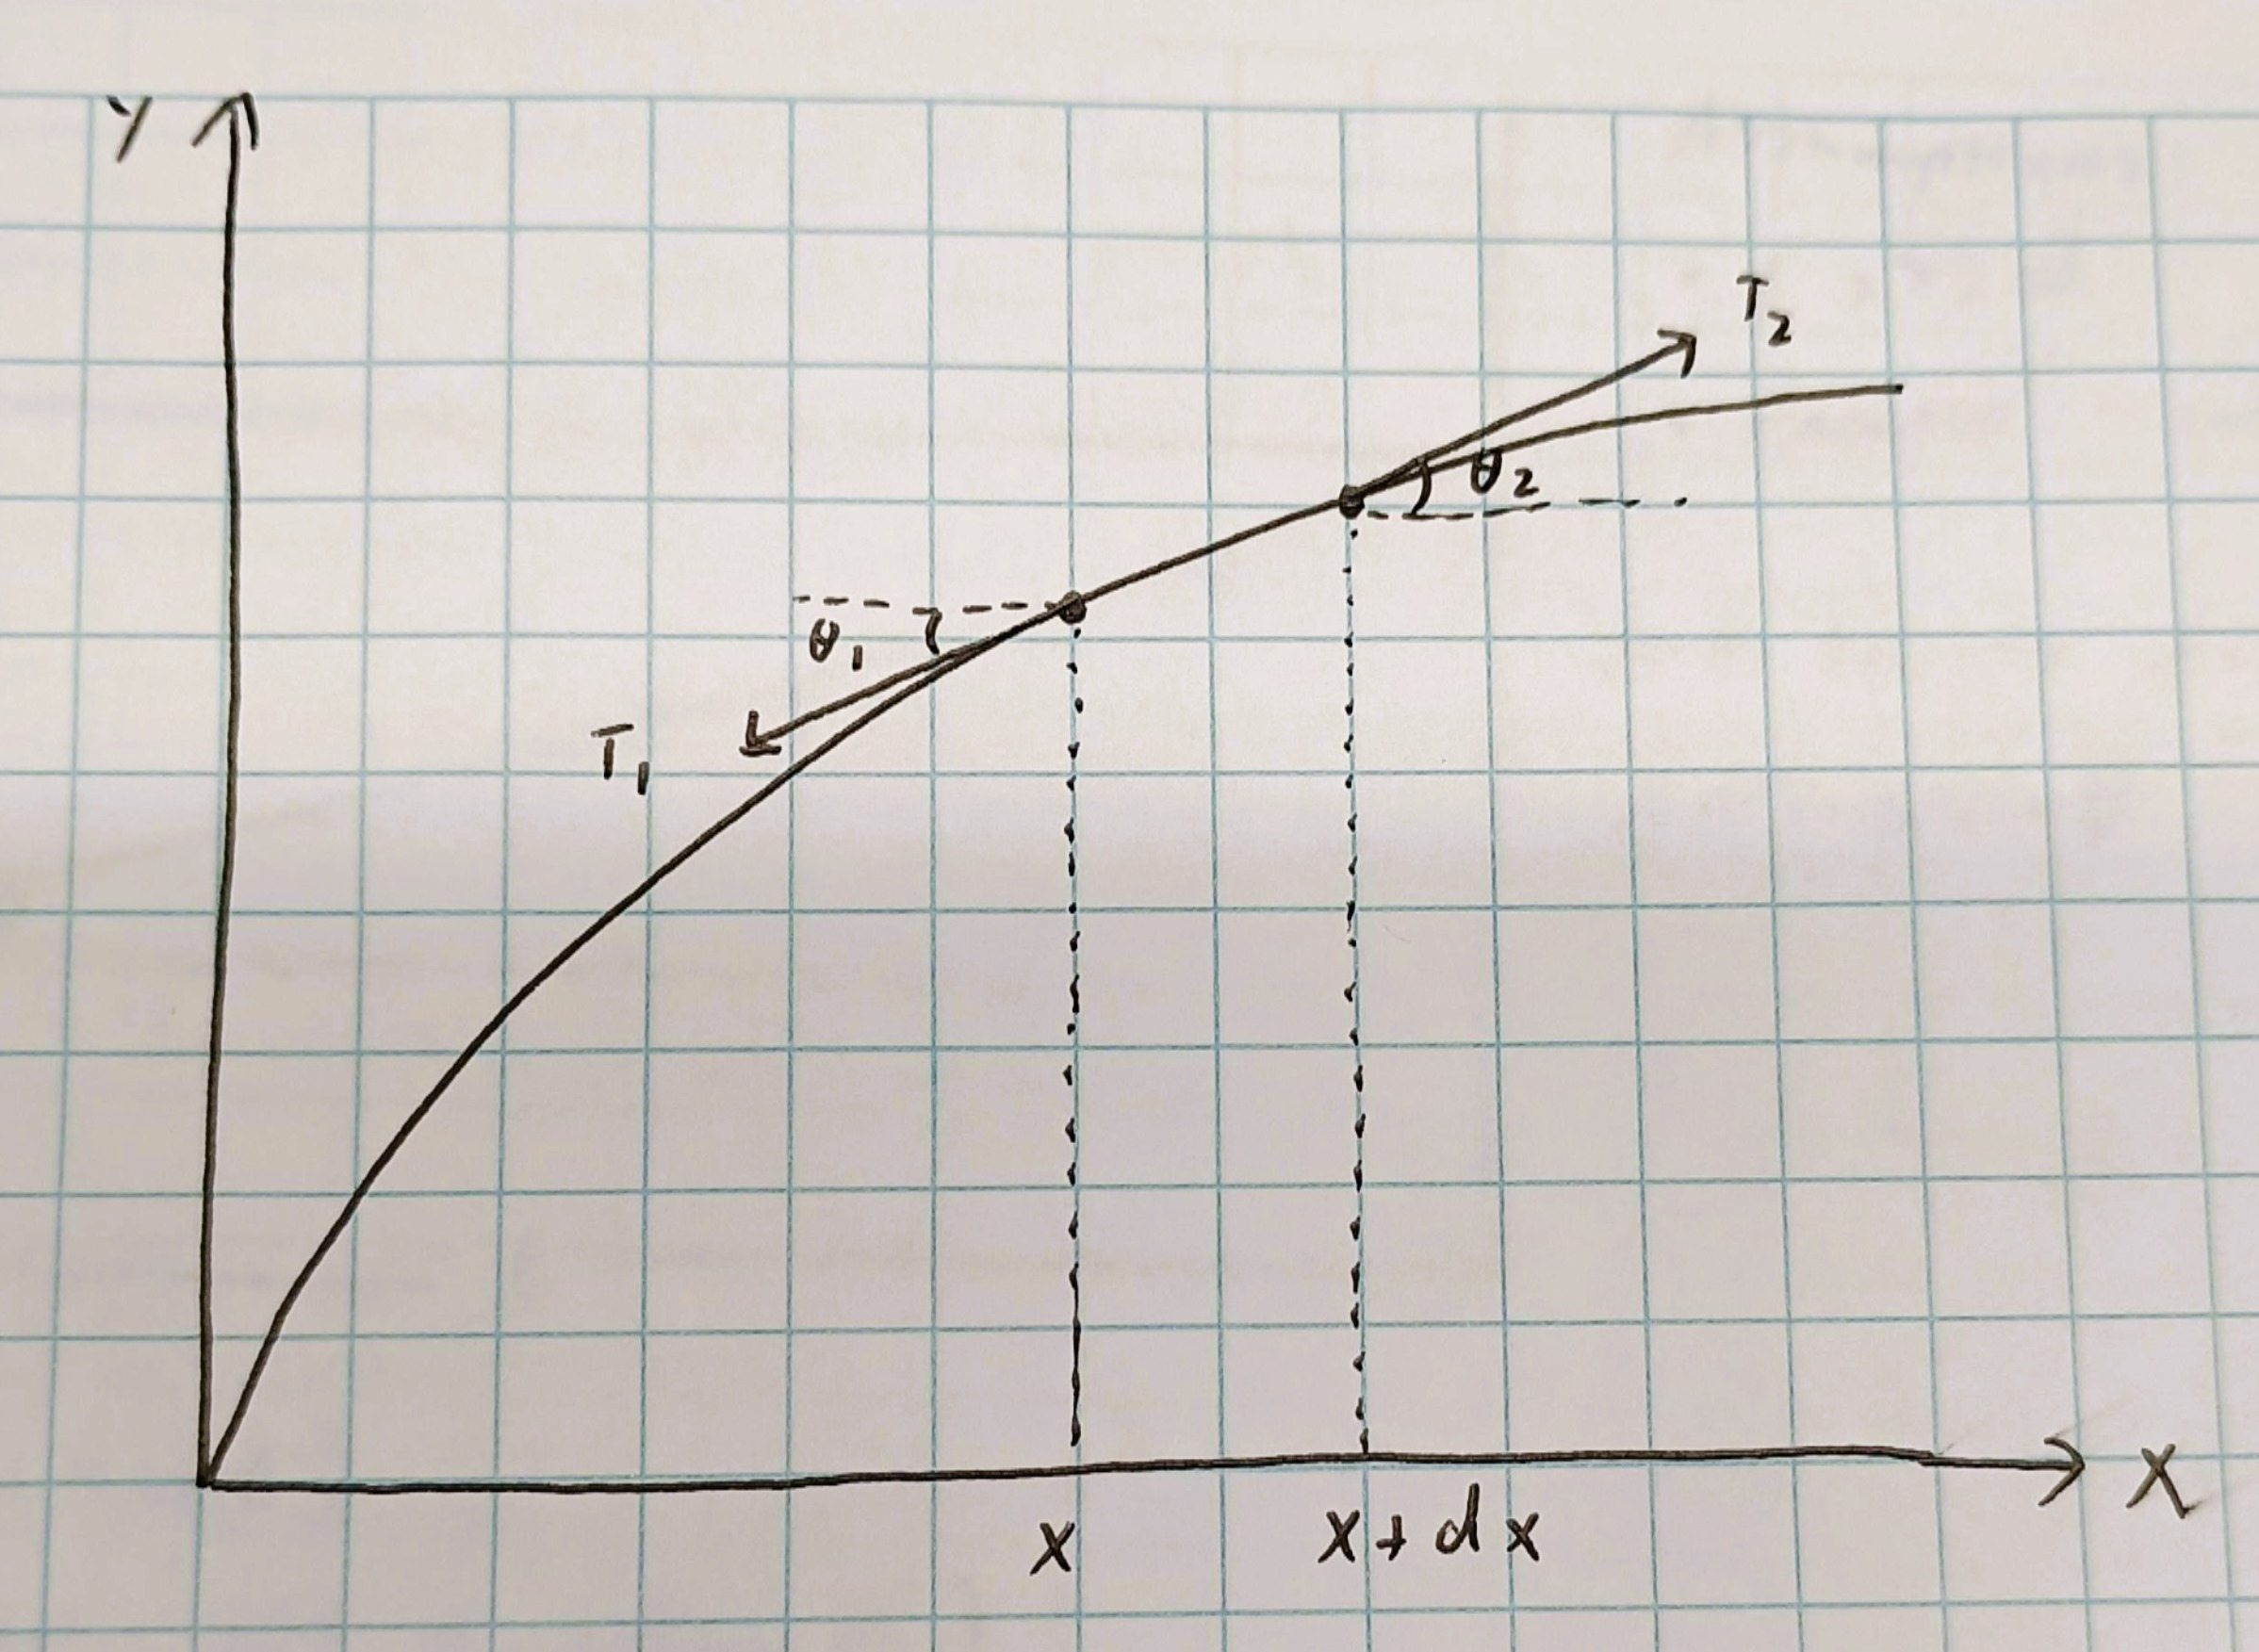
\includegraphics[width=0.6\textwidth]{String.jpg}
\end{figure}
\[
\text{where }\theta_1 = \theta(x), \quad \theta_2 = \theta(x+dx), \quad dm = \mu \, dx 
\]
\underline{In y:}
\[
\sum F_y = dm \, a_y
\]
\[
T_2 \sin \theta_2 - T_1 \sin \theta_1 = (\mu \, dx \,) \frac{d^2 y}{dt^2}
\]
By small angle approx $\sin \theta \approx \theta \approx \tan \theta$ and $\tan \theta = dy/dx$
\[
T_2 \left.\frac{dy}{dx}\right|_{x+dx} - T_1 \left.\frac{dy}{dx}\right|_{x} = \mu \, dx \, \frac{d^2 y}{dt^2}
\]
\underline{In x}
\[
\sum F_x = dm \, a_x, \quad a_x = 0
\]
\[
T_2 \cos \theta_2 - T_1 \cos \theta_1 = 0 
\quad \text{with small-angle approx } \cos \theta \approx 1
\]
\[
T_1 = T_2
\]
Thus,
\[
T \left( \frac{\left.\frac{dy}{dx}\right|_{x+dx} - \left.\frac{dy}{dx}\right|_{x}}{dx} \right) = \mu \frac{d^2 y}{dt^2}
\]
\[
\boxed{T \frac{d^2 y}{dx^2} = \mu \frac{d^2 y}{dt^2}}
\]
    \item Sound Waves
\\The physics of the phenomenon of sound waves involves three features:
\begin{enumerate}
    \item The gas moves and changes its density.
    \item The change in density corresponds to a change in pressure.
    \item Pressure differences generate gas motion.
\end{enumerate}

\begin{figure}[H]
    \centering
    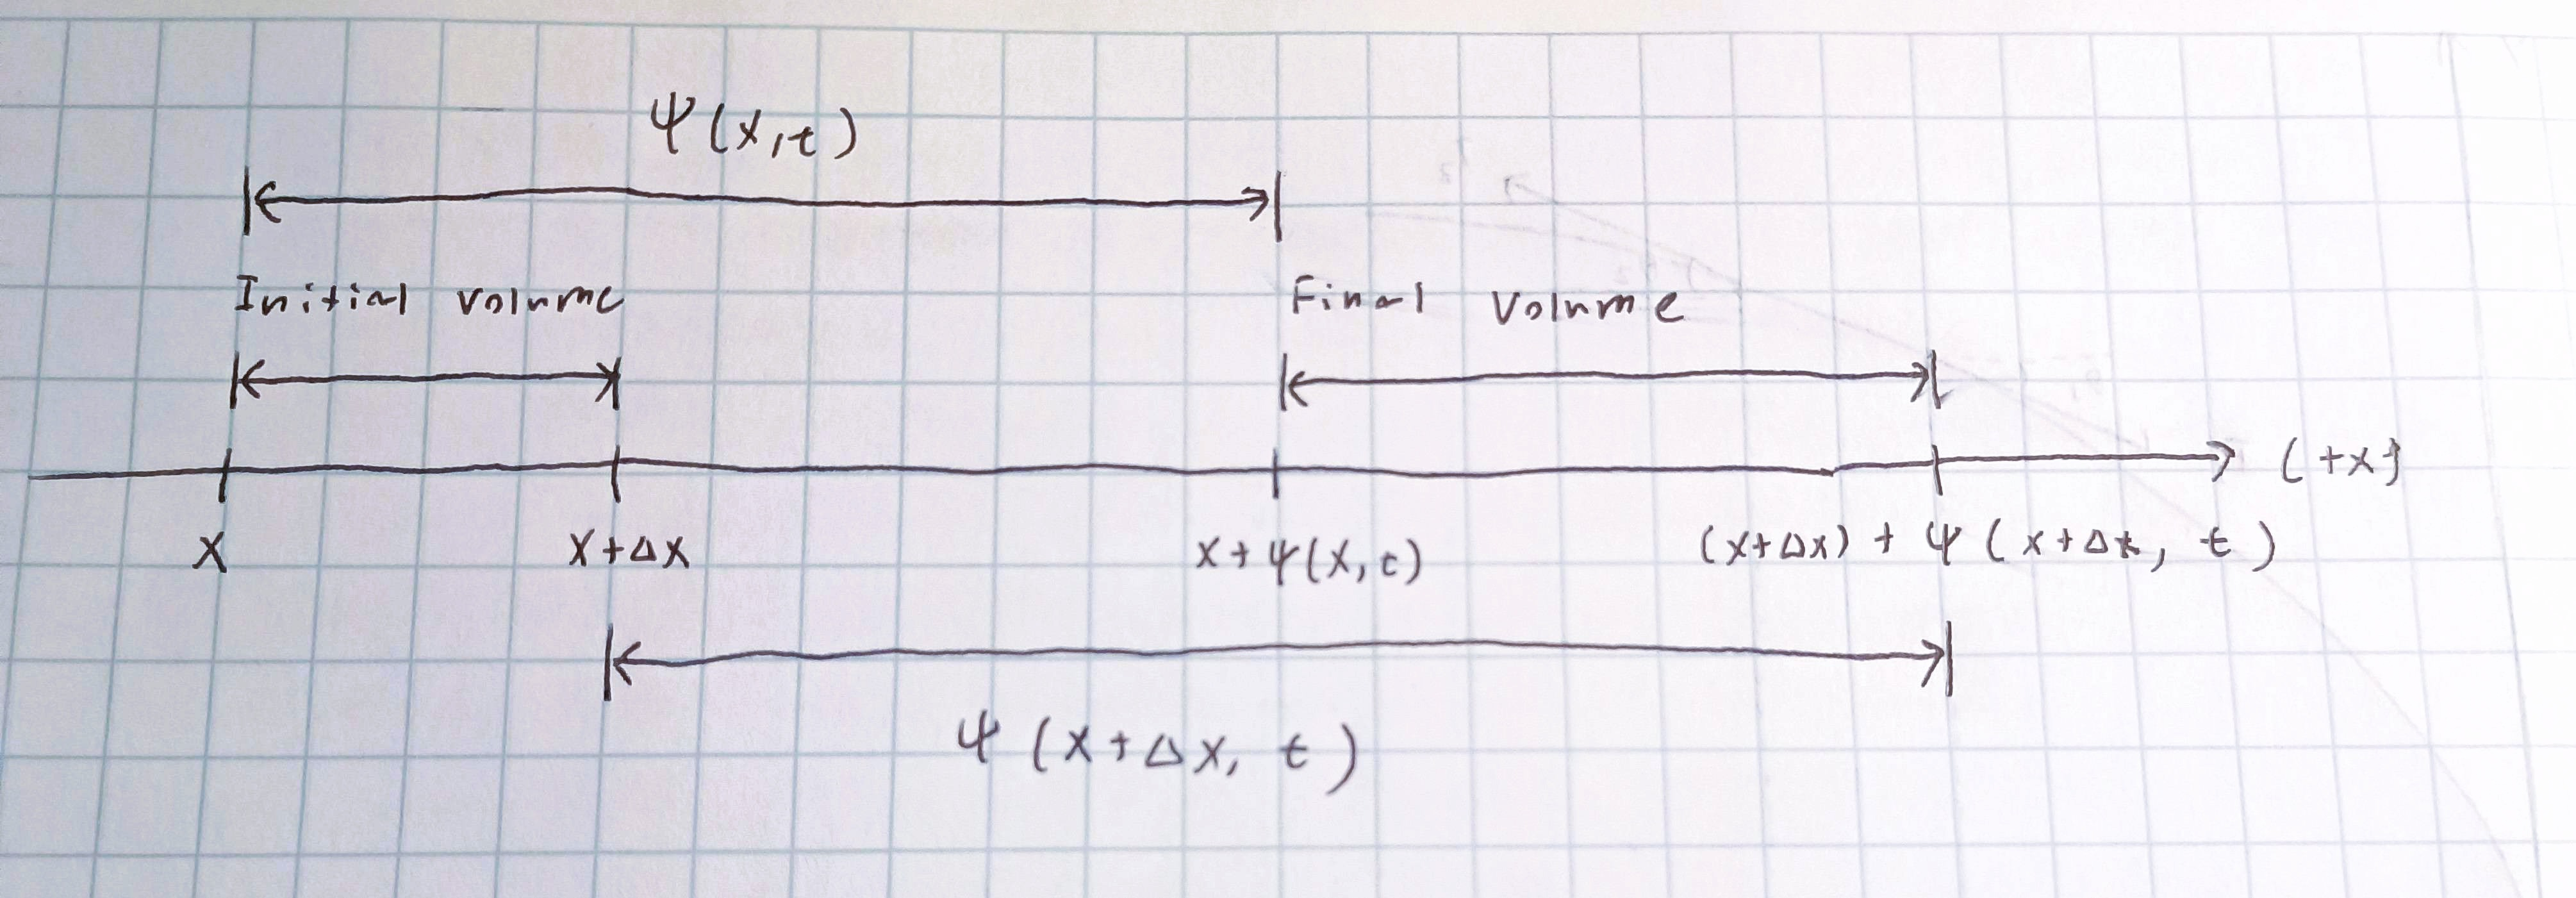
\includegraphics[width=1\textwidth]{Sound.JPG}
    \caption{The displacement of the air particles initially at $x$ is $\psi(x,t)$, and at $x+\Delta x$ it is $\psi(x+\Delta x,t)$.}
\end{figure}
\begin{align*}
\text{Initial Volume} &= A \big[(x + \Delta x) - x\big] = A \, \Delta x
\\ \text{Final Volume} &= A \Big[ (x + \Delta x + \psi(x + \Delta x, t)) - (x + \psi(x, t)) \Big] \\
&= A (\Delta x + \Delta \psi)
\end{align*}
By conservation of mass (mass before and after the wave passes are equal)
\\  Where:
\begin{itemize}
    \item $A =$ Cross-sectional area of air
    \item $V_0 =$ Initial volume
    \item $\rho_0 =$ Initial density
\end{itemize}
\[
\rho_0 A \, dx = (\rho_0 + d\rho) A \, (dx + d\psi)
\]
\[
\rho_0 \, dx = (\rho_0 + d\rho) \left( 1 + \frac{d\psi}{dx} \right) dx
\]
\[
\rho_0 \ = (\rho_0 + d\rho) \left( 1 + \frac{d\psi}{dx} \right) 
\]
\[
\rho_0 \, = \rho_0 \, + \rho_0 \frac{d\psi}{dx} + d\rho \,  + d\rho \frac{d\psi}{dx} \quad \text{$d\rho$ is small so it reduces to 0}
\]
\begin{equation}
\boxed{d\rho = - \rho_0 \frac{d\psi}{dx}}
\label{1}
\end{equation}
This equation is what we would expect physically. If the displacements vary with $x$, then there will be density changes. The sign is also correct: if the displacement $\psi$ increases with $x$, so that the air is stretched out, the density must decrease.

\vspace{1em} Also by conservation of mass
\[
\rho_0 V_0 = (\rho_0 + \Delta \rho)(V_0 + \Delta V)
\]
\[
\Delta \rho \, V_0 = - \rho_0 \, \Delta V
\]
\[
\frac{\Delta \rho}{\rho_0} = - \frac{\Delta V}{V_0}
\]
Substitute into
\[
B = - \frac{\Delta P}{\Delta V / V}
\]
\[
B = \frac{\Delta P}{\Delta \rho / \rho_0}
\]
\begin{equation}
\boxed{\Delta P = \frac{B}{\rho_0} \, \Delta \rho}
\label{eqn:2}
\end{equation}
We find in this way that the change pressure $\Delta P$ is proportional to the change in density $\Delta \rho$, and we may call the proportionality factor $B/\rho_o$.

\vspace{1em} Force analysis on a region of air
\begin{figure}[H]
    \centering
    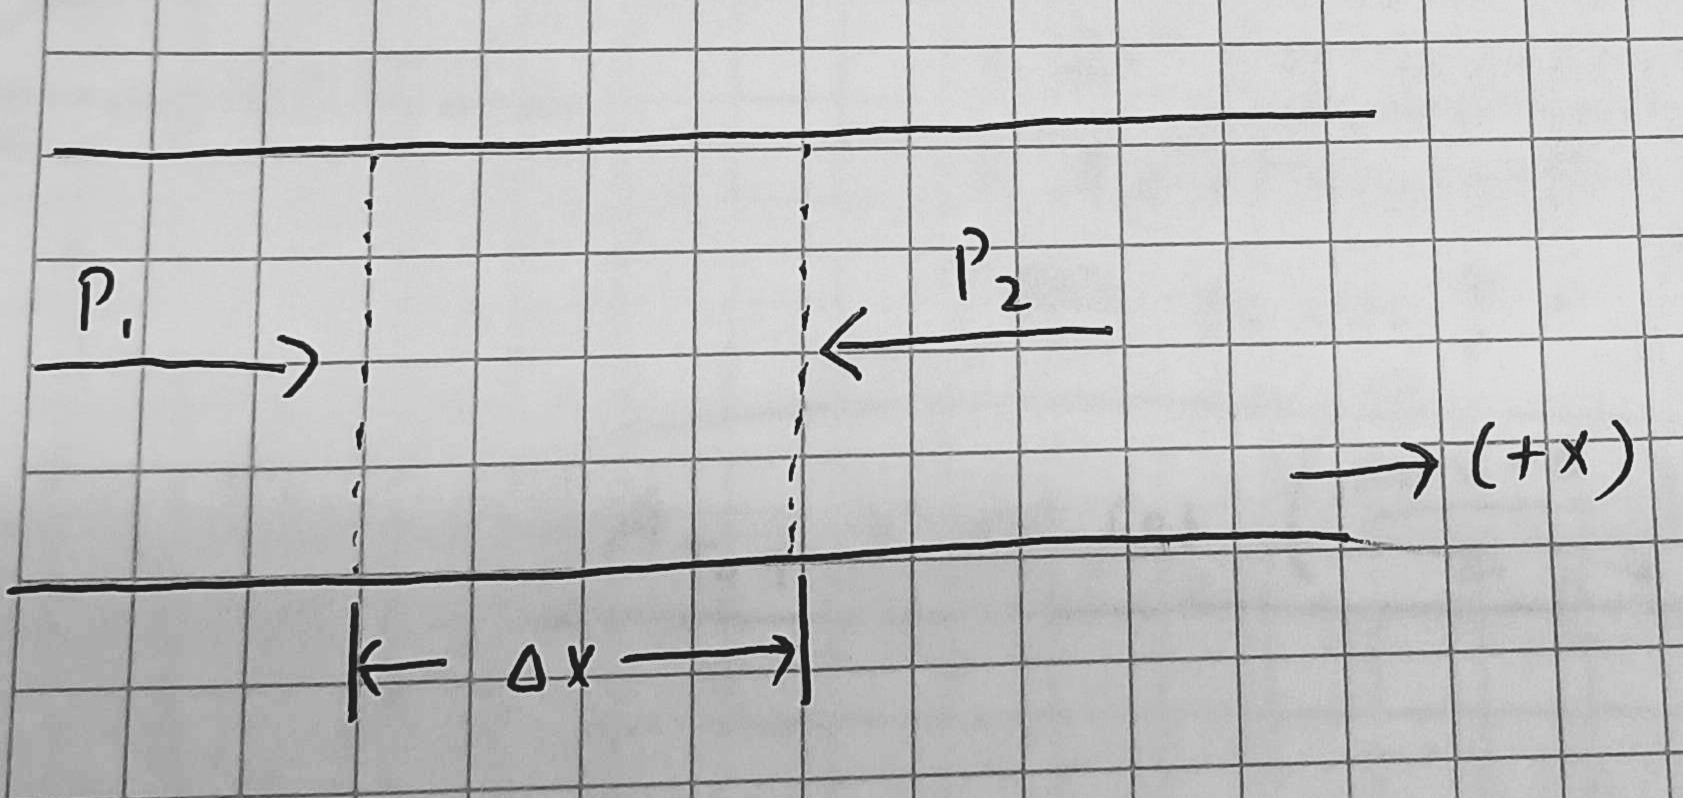
\includegraphics[width=0.5\textwidth]{Sound 2.JPG}
\end{figure}
Where $P_o$ = Pressure in region
\begin{align*}
\sum F \;&=\; m a \\
P_1 A - P_2 A \;&=\; \rho_0 A \, dx \, \frac{d^2 \psi}{dt^2} \\
(P_0 + \Delta P_1) A - (P_0 + \Delta P_2) A \;&=\; \rho_0 A \, dx \, \frac{d^2 \psi}{dt^2} \\
\Delta P_1 - \Delta P_2 \;&=\; \rho_0 \, dx \, \frac{d^2 \psi}{dt^2}, \quad 
\left( \Delta P_2 - \Delta P_1 = \frac{d (\Delta P)}{dx} \, dx \right) \\
- \frac{d (\Delta P)}{dx} \, dx \;&=\; \rho_0 \, dx \, \frac{d^2 \psi}{dt^2} \\
\rho_0 \frac{d^2 \psi}{dt^2} \;&=\; - \frac{d}{dx} \left( \frac{B}{\rho_0} d \rho \right) \quad \text{Plug in eqn (1)} \\
\rho_0 \frac{d^2 \psi}{dt^2} \;&=\; - \frac{d}{dx} \left( \frac{B}{\rho_0} \left(-\rho_0 \frac{d\psi}{dx} \right) \right) \quad \text{Plug in eqn (2)} \\
\end{align*}
\[\boxed{\rho_0 \frac{d^2 \psi}{dt^2} = B \frac{d^2 \psi}{dx^2}}\]
\end{itemize}

    \item Understand the properties of the wave equation and be able to prove the general solution to the wave equation works. Determine whether a given function is a solution to the wave equation, prove the principal of superposition for waves, and describe qualitatively and quantitatively such superpositions.
    \item Use phasor diagrams (or algebraically use complex exponentials) to calculate the superposition of sinusoidal waveforms.
\newpage
    \item Express solutions to the wave equation in terms of trigonometric functions and be able to define the transverse velocity, phase velocity, angular frequency, wavenumber, phase shift of a wave, wave speed, wavelength, period, etc.
\begin{itemize}
     \item Waves on a string has the form
\[
y(x,t) = y_m \sin(kx \pm \omega t + \phi)
\]
Where
    \begin{itemize}
\item $y_m$ is the amplitude
\item k is the angular wave number (spatial frequency: measures how many oscillations per wavelength in $[rad/m]$
\item $\omega$ is the angular frequency in $[rad/s]$
\item $(kx \pm \omega t+\phi)$ is the phase with a phase shift of $\phi$
    \end{itemize}
\[
k = \frac{2 \pi}{\lambda}
\]
\[
\frac{\omega}{2\pi} = f = \frac{1}{T} \; [\text{Hz}]
\]
The wave travels with a phase velocity
\[
v = \frac{\omega}{k} = \frac{\lambda}{T} = \lambda f
\]
\[
v_{string} = \sqrt{\frac{\tau}{\mu}}
\]
and has a transverse velocity of
\[
\frac{\partial y}{\partial t} = \pm y_m \, \omega \, \cos(kx \pm \omega t + \phi)
\]
\item Similarly, sound waves has the form
\[
s(x,t) = s_m \cos(kx \pm \omega t + \phi)
\]
where $s_m$ is the displacement amplitude from the equilibrium.\\
The sound wave also carries a pressure change of the medium from equilibrium pressure
\[
\Delta P = \Delta P_m \sin(kx \pm \omega t + \phi)
\]
where the pressure amplitude $\Delta P_m$ is
\[
\Delta P_m = v \, \rho \,  \omega \, s_m
\]
\[\implies s_m = \frac{\Delta p_m}{v \, \rho \, \omega} = \frac{\Delta p_m}{Bk}\]
The sound wave travels with a phase velocity
\[
v_{\text{sound}} = \sqrt{\frac{B}{\rho}}, \quad \text{where} \quad B = - \frac{\Delta P}{\Delta V / V}
\]
Note: Speed of sound in air at 20$^\circ$C is 343 m/s
\end{itemize}    
    \item Define the impedance of a wave, describe its physical significance and relation to reflection and transmission of waves.
\begin{itemize}
    \item Impedance is a physical property of a wave medium that relates the force (or pressure) to the particle velocity in a wave. When a wave encounters a boundary between two media with different impedances, part of the wave is reflected. This reflection occurs because the difference in impedance ensures that the forces and wave speeds at the boundary are balanced, maintaining continuity of motion and energy across the interface.
\\For strings:
\[
Z = \mu \, v = \sqrt{\mu T}
\]
\[
F_y =  Z \frac{\partial y}{\partial t}
\]

For sound waves moving through air:
\[
Z = \rho \, v = \sqrt{\rho B}
\]
\[
\Delta P =  Z \, \frac{\partial s}{\partial t}
\]
\end{itemize}
    \item Describe the boundary conditions that must be satisfied an interface between two media. Use those conditions to determine the reflectance and transmittance of a wave through the interface.
\begin{itemize}
    \item \textbf{Set up:}
    \begin{figure}[H]
    \centering
    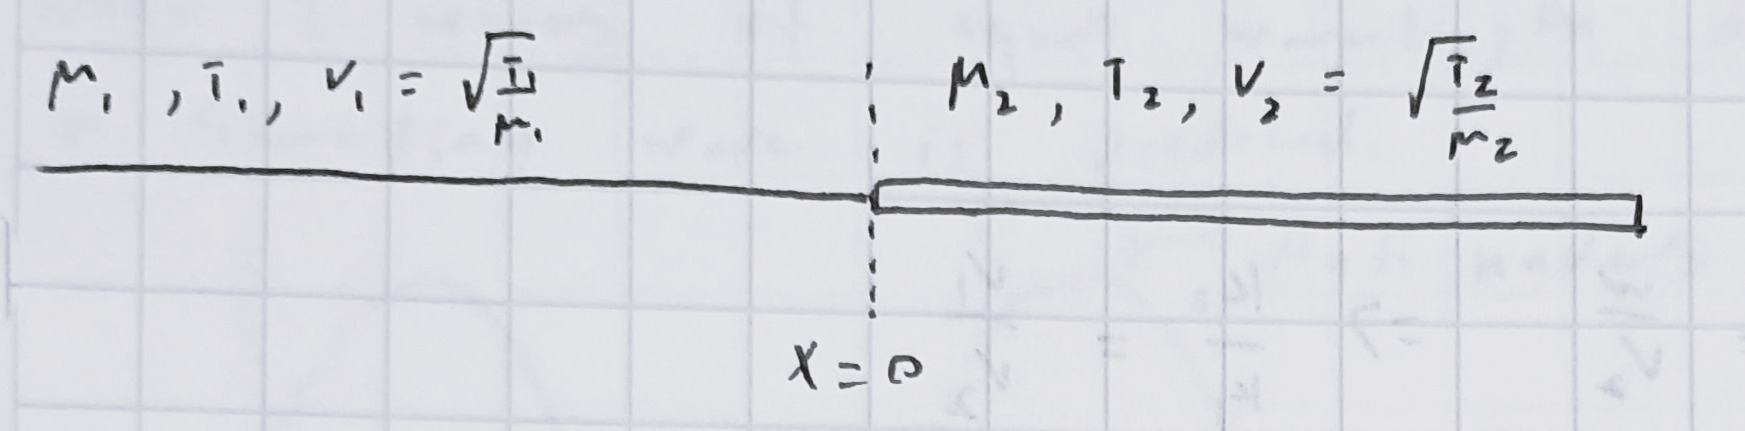
\includegraphics[width=0.8\textwidth]{Reflection 1.JPG}
    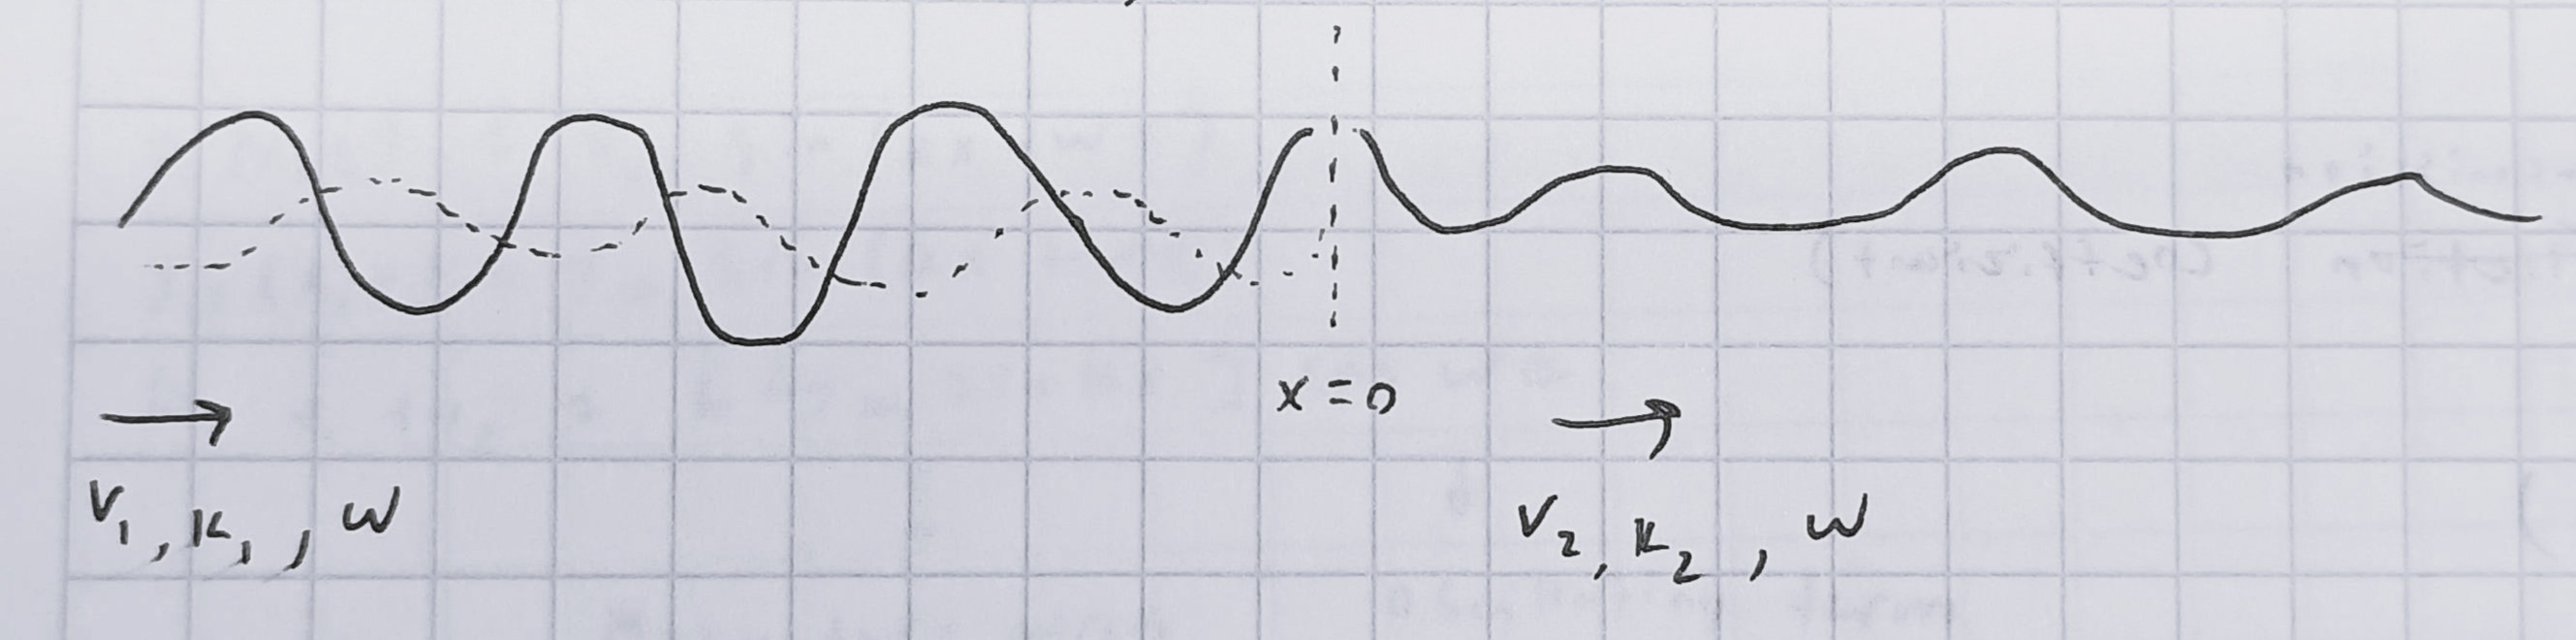
\includegraphics[width=0.8\textwidth]{Reflection 2.JPG}
    \end{figure}
    \begin{itemize}
        \item Tension must be equal or else the string will be pulled to one side
        \item $\omega_1=\omega_2$ as is $f_1=f_2$ because it is determined by the source of the wave
        \item $\lambda_1 \neq \lambda_2$ since wave velocity is not equal but frequency is equal ($v=\lambda f$)
        \item $k_1 \neq k_2$ since wavelengths are not equal
    \end{itemize}
    Wave in medium 1: $y_{incident}+y_{reflected}$
    \[y_1(x,t) = y_Icos(k_1x-\omega t)+y_Rcos(k_1x+\omega t)\]
    ($y_R$ has the same wavenumber since wave speeds are equal within the same medium and f)
    \\ Wave in medium 2: $y_{transmitted}$
    \[y_2(x,t)=y_Tcos(k_2x-\omega t)\]
    \item \textbf{Boundary conditions at x=0:}
    \begin{itemize}
    \item String is continuous (total transverse displacement at x=0 for all time is equal for both mediums)
    \[y_1(0,t)=y_2(0,t)\]
    \[y_I(0-\omega t)+y_Rcos(0+\omega t)=y_Tcos(0-\omega t)\]
    \[y_I+y_R=y_T \quad \text{$cos((\omega t)$ cancels out)}\]
    \item The slope is continuous at x=0 (if slopes are not equal, tension will not cancel out)
    \[\left.\frac{dy_1}{dx}\right|_{x=0} \;=\; \left.\frac{dy_2}{dx}\right|_{x=0}\]
    \[
\left. \bigl(- y_I k_1 \sin(k_1 x - \omega t) - y_R k_1 \sin(k_1 x + \omega t)\bigr) \right|_{x=0}
=
\left. \bigl(- y_T k_2 \sin(k_2 x - \omega t)\bigr) \right|_{x=0}
\]
\[
- y_I k_1 \sin(-\omega t) \;-\; y_R k_1 \sin(\omega t) 
= - y_T k_2 \sin(-\omega t)
\]
\[y_Ik_1-y_Rk_1=y_Tk_2 \quad \text{($sin(\omega t)$ cancels out)}\]   
    \end{itemize}
\item \textbf{Solve system of equations for $y_T/y_I$ and $y_R/y_I$}
\[\boxed{y_T=\frac{2v_2}{v_1+v_2}y_I \quad \text{(Transmission coefficient)}}\]
\[\boxed{y_R=\frac{v_2-v_1}{v_1+v_2}y_I \quad \text{(Reflection coefficient)}}\]
Note: If T=transmission coefficient and R=reflection coefficient then 1+R=T
\end{itemize}
    \item Determine the resonance condition for standing waves on strings, closed ended pipes, open-ended pipes, etc. For the same situations be able to relate wavelengths, frequencies, phase velocities and solve for unknown quantities.
\begin{itemize}
    \item \textbf{Standing waves} are formed when two waves of the same frequency and amplitude travel in opposite directions and interfere.
    \\Let
    \[y_1(x,t)=y_msin(kx-\omega t)\]
    \[y_2(x,t)=y_msin(kx+\omega t)\]
    \[y_1+y_2 = [2y_msin(kx)]cos(\omega t)\]
    The amplitude is determined by $2y_msin(kx)$ thus there will be a node when $sin(kx)=0$ and an antinode when $sin(kx)=1$
    \\ Setting $kx=n\pi$
    \[x=n \frac{\lambda}{2} \quad \text{x positions for nodes}\]
    \\ Setting $kx=(n+\frac{1}{2})\pi$
    \[x=\left(n+\frac{1}{2}\right)\frac{\lambda}{2} \quad \text{x positions for antinodes}\]
    \item \textbf{Strings fixed at both ends separated by length L}
    \begin{figure}[H]
    \centering
    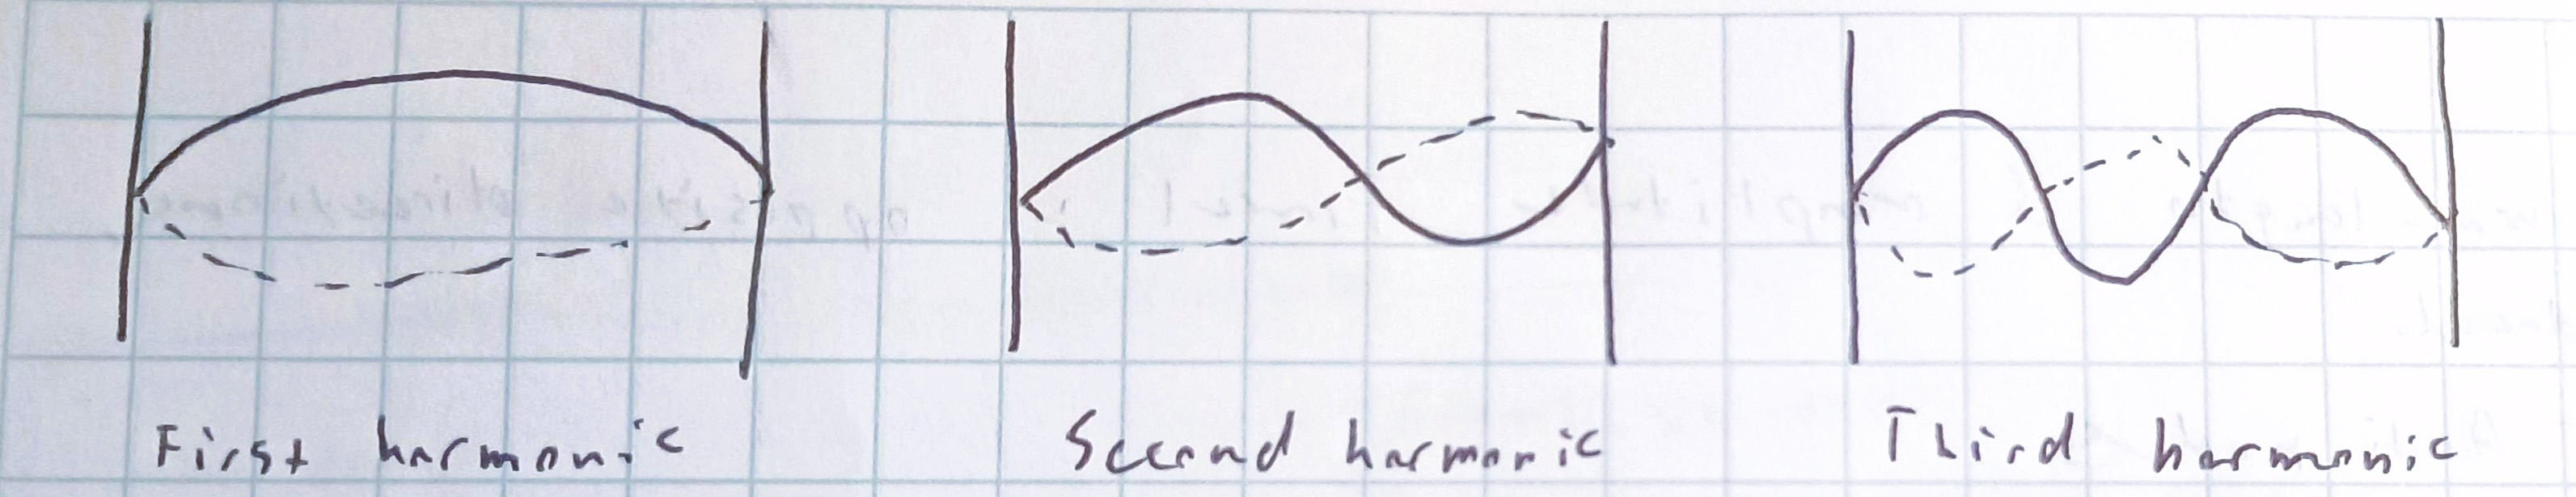
\includegraphics[width=1\textwidth]{String Harmonics.jpg}
    \end{figure}
    \[\boxed{\lambda=\frac{2L}{n}} \quad \text{Where n is the harmonic number}\]
    \[\boxed{f_{resonant}=\frac{v}{\lambda}=\frac{nv}{2L}}\]
    The first harmonic is also called the fundamental frequency.
    \newpage
    \item \textbf{Pipes open at both ends separated by length L (same as strings fixed at both ends)}
    \begin{figure}[H]
    \centering
    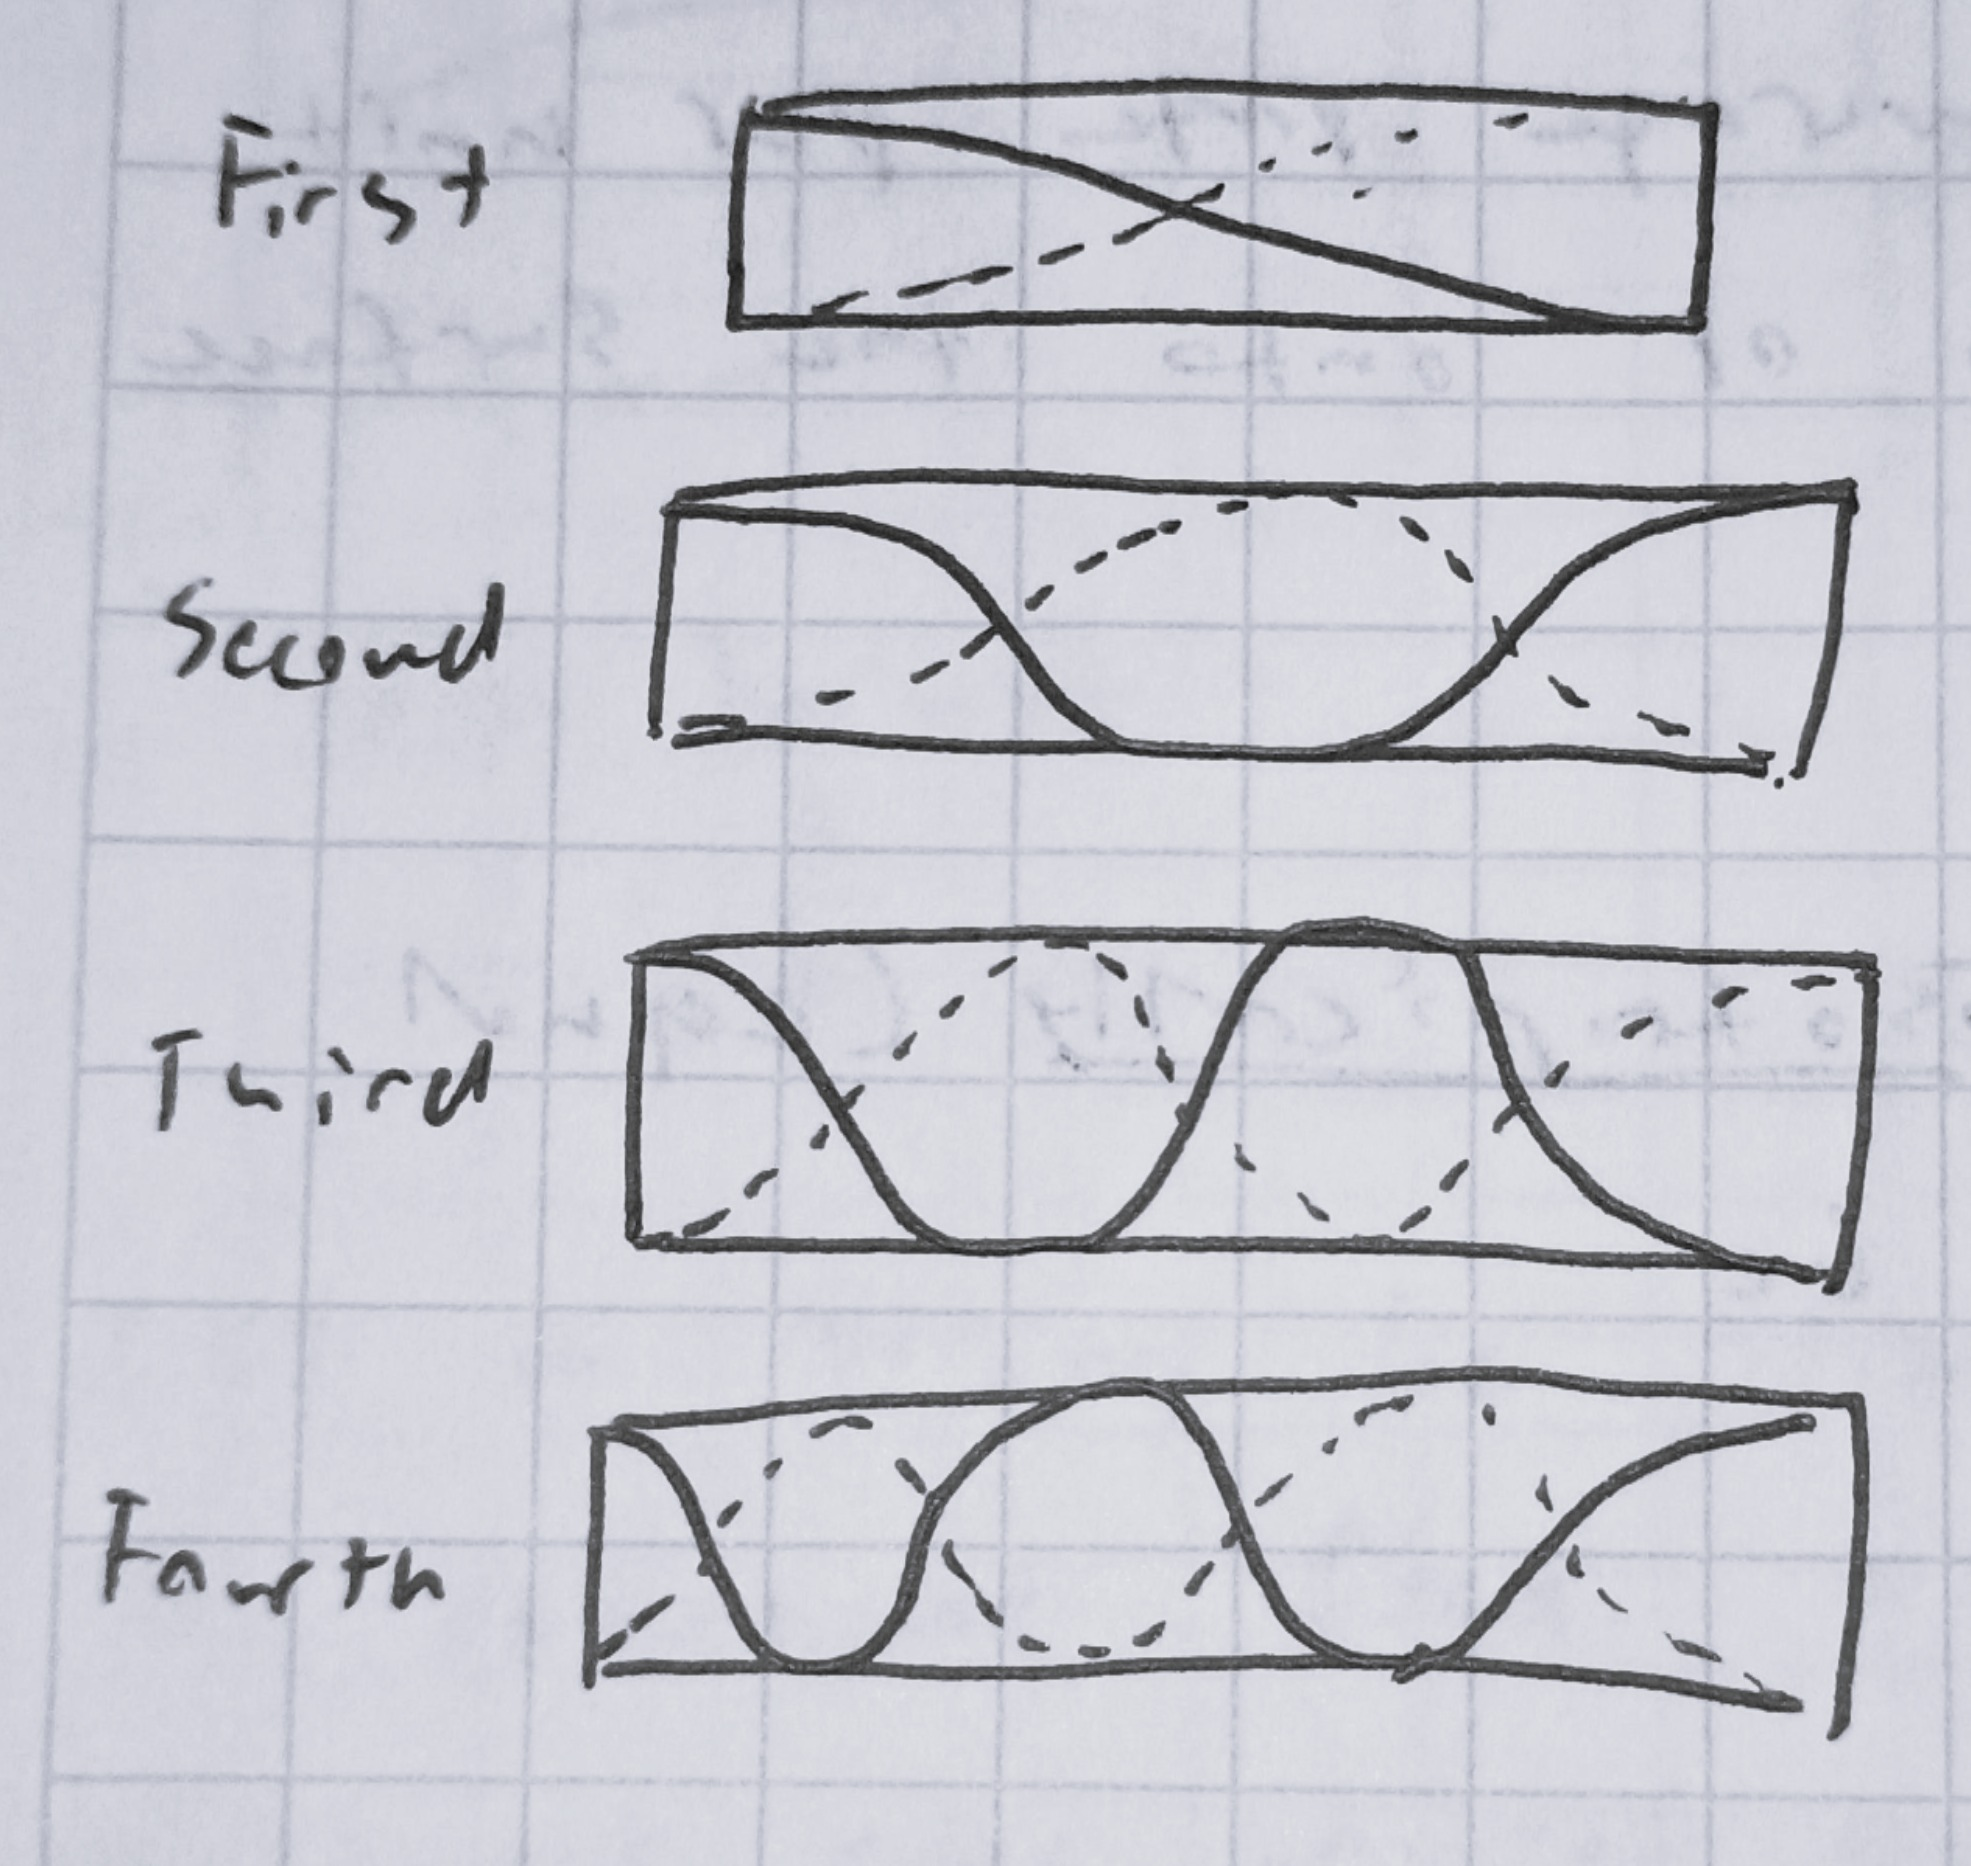
\includegraphics[width=0.4\textwidth]{Pipe open.jpg}
    \end{figure}
    \[\boxed{\lambda=\frac{2L}{n}}\]
    \[\boxed{f_{resonant}=\frac{v}{\lambda}=\frac{nv}{2L}}\]
    \item \textbf{Pipes closed at one end separated by length L (ONLY odd harmonics)}
   \begin{figure}[H]
    \centering
    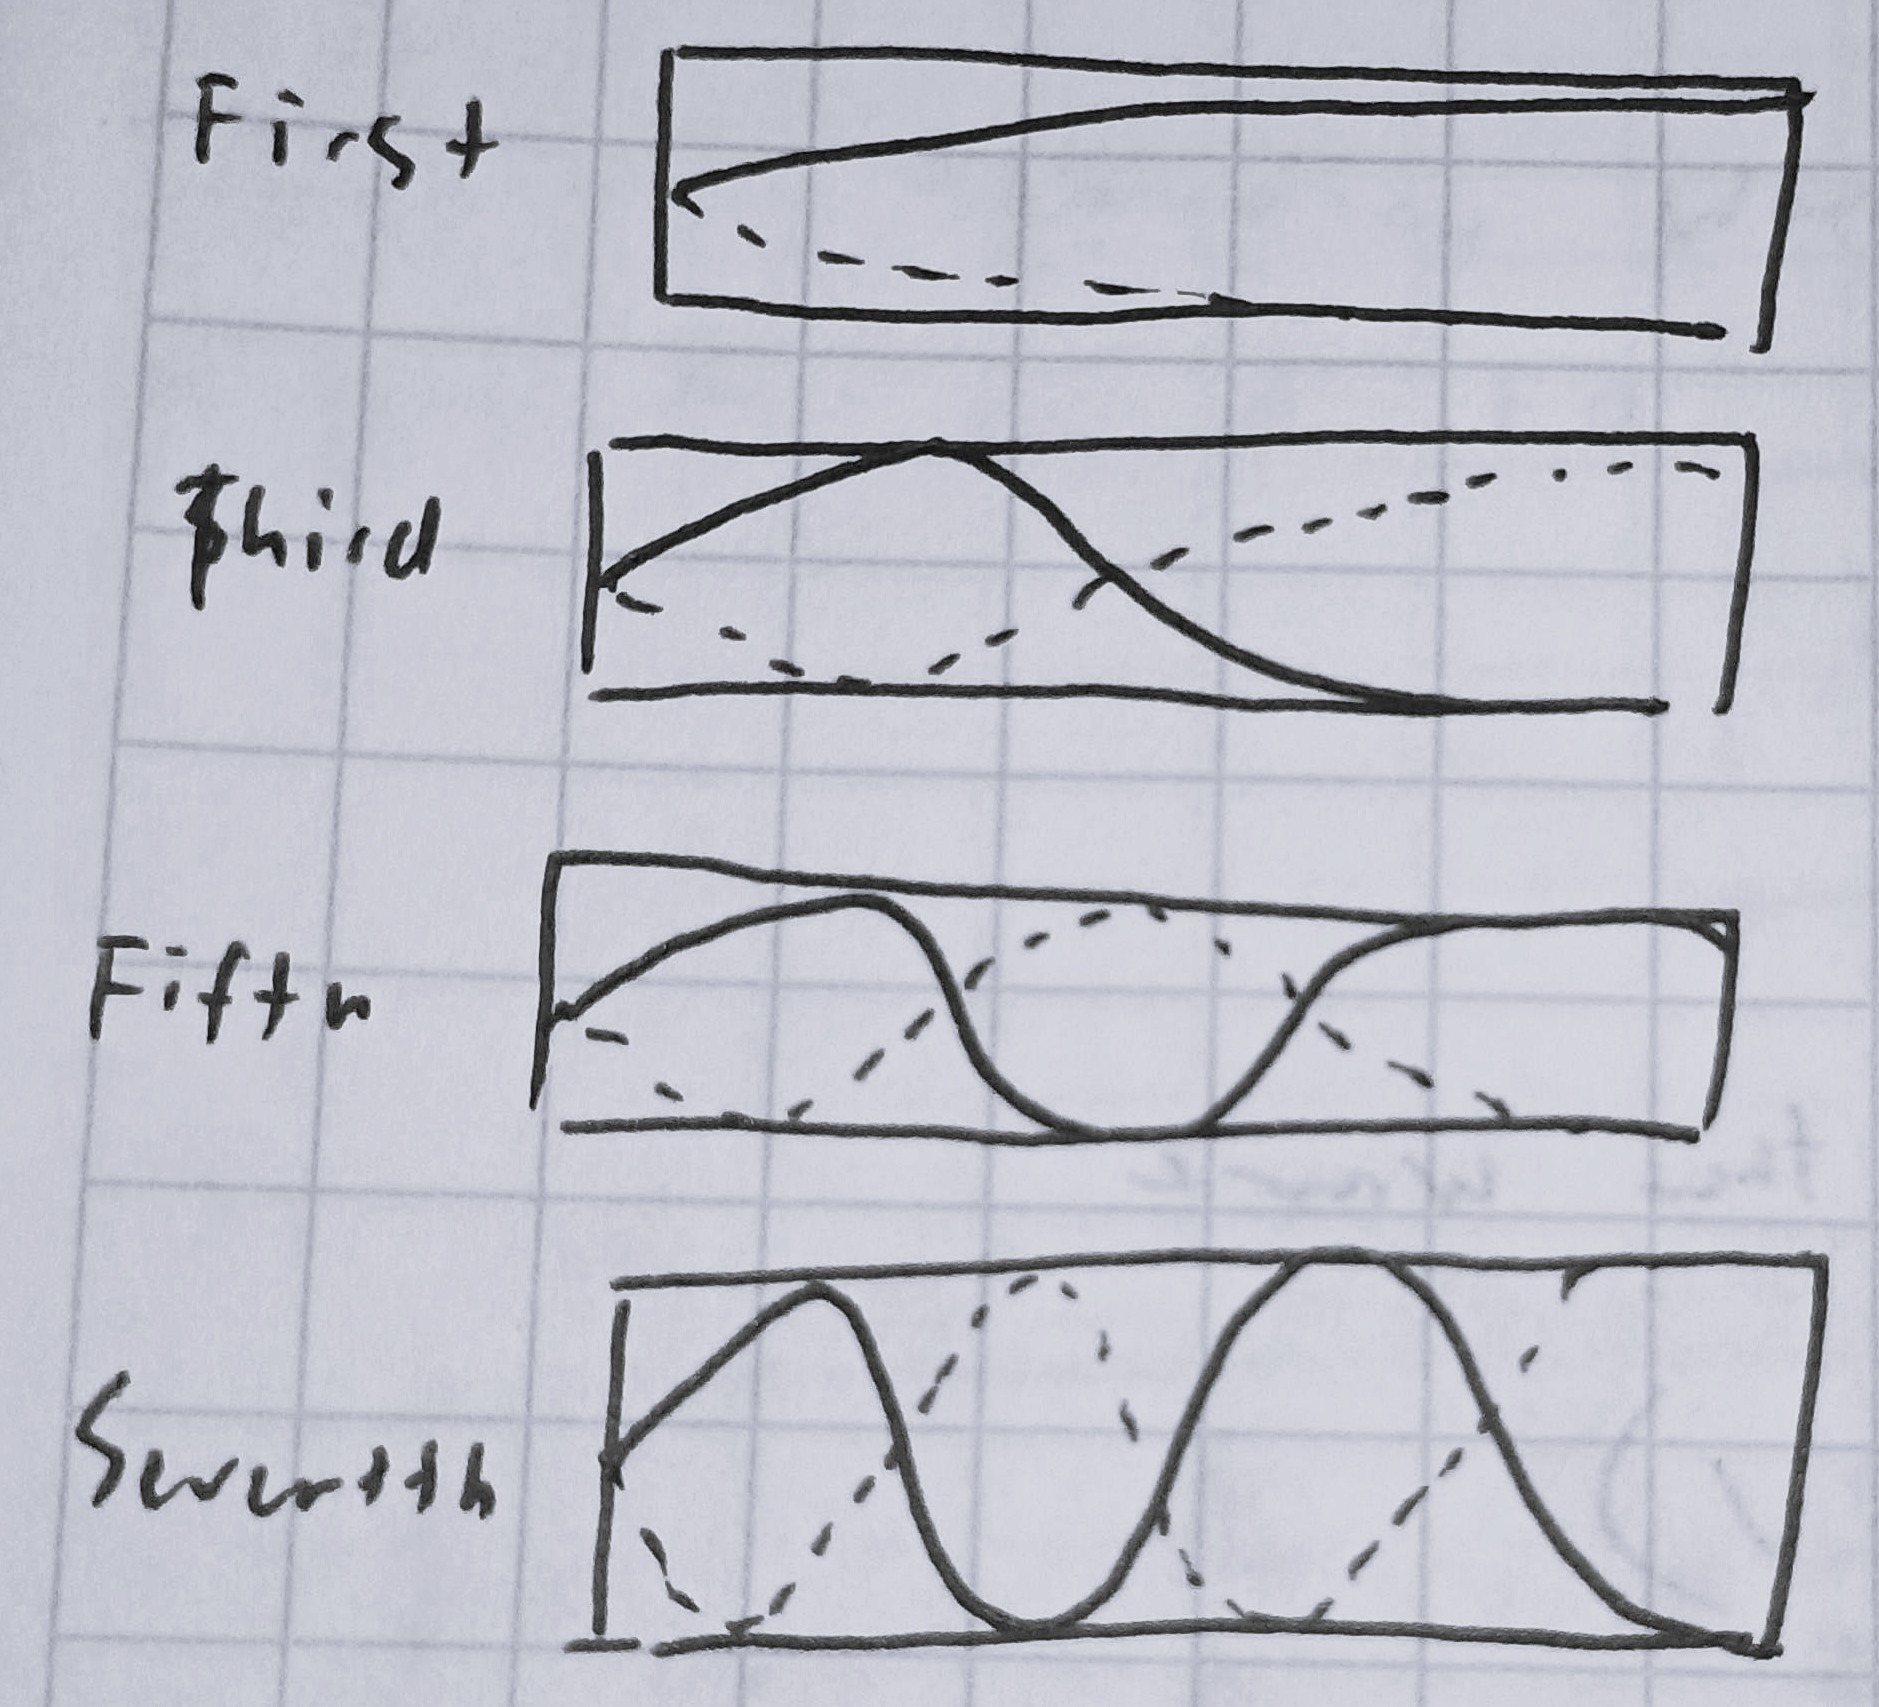
\includegraphics[width=0.4\textwidth]{Pipe closed.jpg}
    \end{figure}
    \[\boxed{\lambda=\frac{4L}{n}} \quad \text{Where n is odd (1,3,5...)}\]
    \[\boxed{f_{resonant}=\frac{v}{\lambda}=\frac{nv}{4L}}\]
\end{itemize}
\newpage
    \item Explain what a beat is, when it occurs, and derive the beat frequency.
\begin{itemize}
    \item A beat is formed when two waves of slightly different frequencies interfere. The resulting wave oscillates at a frequency that is the average of the two original frequencies, but its amplitude varies at a rate equal to the difference between the two frequencies. 
    \begin{figure}[H]
    \centering
    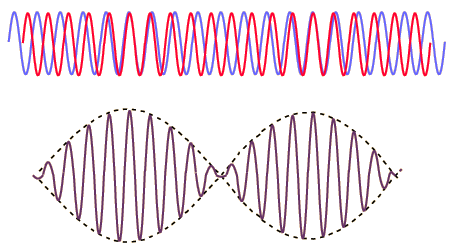
\includegraphics[width=0.4\textwidth]{beat4.png}
    \end{figure}
    Let
    \[s_1(t)=s_mcos(\omega_1 t)\]
    \[s_2(t)=s_mcos(\omega_2 t)\]
    \[s_1+s_2 = \left[2s_mcos(\omega't)\right]cos(\omega t)\]
    Where $\omega'= (\omega_1-\omega_2)/2$ (half the difference in angular freq) and $\omega=(\omega_1+\omega_2)/2$ (the average angular freq)
    \[\boxed{f_{beat} = f_1 - f_2}\]
\end{itemize}
    \item Know the average wave power carried by a wave on a string.
\begin{itemize}
    \item \[W=F_y dy\]
     \[P=\frac{W}{\Delta t}=F_y \frac{dy}{dt}\]
    For a wave on a string:
    \[P=\left(Z \frac{\partial y}{\partial t}\right) \frac{\partial y}{\partial t}\]
    Say $y=y_mcos(kx-\omega t)$
    \[P=Zy_m^2\omega ^2 sin^2(kx-\omega t)\]
    \[P_{average}=\frac{1}{2}Zy_m^2\omega^2\]
    Note: $Z=\mu v$ and the average of $sin^2$ and $cos^2$ over one period is 1/2
\newpage
\end{itemize}
    \item Describe the relation between intensity and amplitude. Write an equation giving the variation of the intensity with distance from the source for waves on a string or sound waves in air.\\ \\
        Note: For a wave on a string, use cross sectional area for power per unit area and length for power per unit length.
    \[\text{Intensity} = \frac{\text{Average rate of energy delivered (Avg Power)}}{\text{Area that wave spreads out}}\]
    \[I \propto (\text{Amplitude})^2\]
\begin{itemize}
    \item For sound waves:
    \[\text{Intensity} = I = \frac{P_{average}}{4\pi r^2} = \frac{1}{2}\rho v \omega^2 s_m^2\]
    \item Intensity level (in decibels)
    \[\beta = (10 \, dB) \log \left(\frac{I}{I_0}\right)\]
    Where $I_0 = 10^{-12} \, W/m^2$ is reference intensity (usually the threshold of hearing)
\end{itemize}
    \item By considering the effective wavelength and the relative velocity between the waves and the observer, determine the Doppler shift for any combination of moving source, moving detector, and ``wind''.\\ \\
    Consider the following variables:
    \begin{enumerate}
    \item $v_{relative}$: Relative speed between the receiver and the wave fronts. ($v_{sound}\pm v_{receiver}$)
    \item $\lambda_{effctive}$: The distance between two successive wave fronts as measured by the receiver. 
    \[\lambda_{effctive}=(v_{sound} \pm v_{source})T=\frac{v_{sound} \pm v_{source}}{f_{source}}\]
    \end{enumerate} 
    Thus the Doppler frequency can be described by:
    \[f'_{Doppler}=\frac{v_{rel}}{\lambda_{eff}}=\frac{v_{sound}\pm v_{receiver}}{v_{sound} \pm v_{source}}f_{source}\]
    Note: Wind either speeds up or slows down the sound wave fronts, consider this when solving cases with wind.\\\\
    \underline{General rule of thumb:} \\If receiver moves towards the incoming sound waves $\implies$ higher received frequency. \\If receiver moves away from incoming sound waves $\implies$ lower received frequency.
    \newpage
    \item Understand the effects of interference on waves. Calculate a phase difference from path length or delay time differences. Use a phasor diagram to quantitatively and qualitatively describe the observed intensities at any given location. For example, describe the pattern of waves produced by two or more ``slits''. Explain applications of interference, for example the interferometer, spectrometer, and thin films like soap bubbles. (Note - these are in the textbook but may not all have been discussed in class).
    \begin{itemize}
        \item Interference due to path length difference
        \\Suppose in 1D, two waves travel in the same direction but $y_2$ starts a distance d behind $y_1$.
        \[y_1=Acos(kx-\omega t)\]
        \[y_2=Acos(k(x+d)-\omega t)=Acos(kx-\omega t+kd)\]
        Thus, $y_2$ is out of phase with $y_1$ by
        \[\boxed{\phi =kd=\frac{2\pi}{\lambda}d}\]
        \item Interference due to time delay difference
        \\Similarly, if $y_2$ starts a time $\Delta t$ after $y_1$ then
        \[y_2=Acos(kx-w(t+\Delta t))=Acos(kx-\omega t-w\Delta t)\]
        Thus, $y_2$ is out of phase with $y_1$ by
        \[\boxed{\phi =\omega \Delta t}\]
        \item Interference from double slits
\begin{figure}[H]
    \centering
    \begin{minipage}{0.7\textwidth}  
        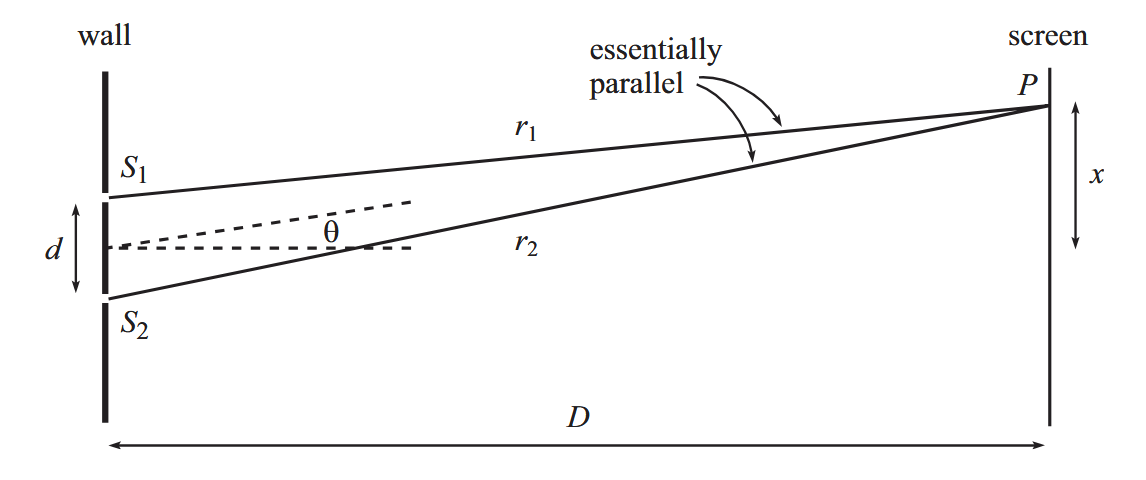
\includegraphics[width=\textwidth]{Double slit 1.png}
    \end{minipage}\hfill
    \begin{minipage}{0.25\textwidth} 
        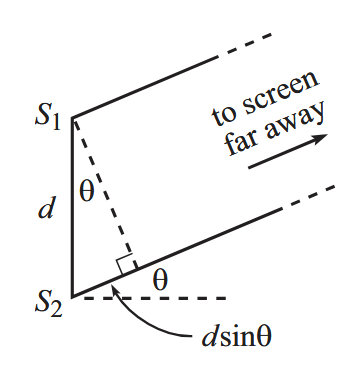
\includegraphics[width=\textwidth]{Double slit 2.png}
    \end{minipage}
\end{figure}
        Assumptions:
        \begin{itemize}
            \item $L \gg d$ (distance to screen is much greater than slit separation)
            \item Parallel lines meet at infinity
        \end{itemize}
        Path length difference:
        \[\Delta L = d sin \theta\]
        Phase difference:
        \[\boxed{\phi = k \Delta L = \frac{2\pi}{\lambda}d sin \theta}\]
        Complete constructive interference (bright fringes):
        \[\phi = kd sin \theta = 2\pi n\]
        \[dsin\theta = n\lambda\]
        Complete destructive interference (dark fringes):
        \[\phi = kd sin \theta = (2n+1)\pi\]
        \[dsin\theta = \left(n+\frac{1}{2}\right)\lambda\]
        Where n is the nth bright/dark fringe from the center
        \item When asked for intensity, use phasor diagram to find resultant amplitude and then use
        \[I \propto A^2\]
        \item \textbf{Example: Triple slit}
\begin{figure}[H]
    \centering
    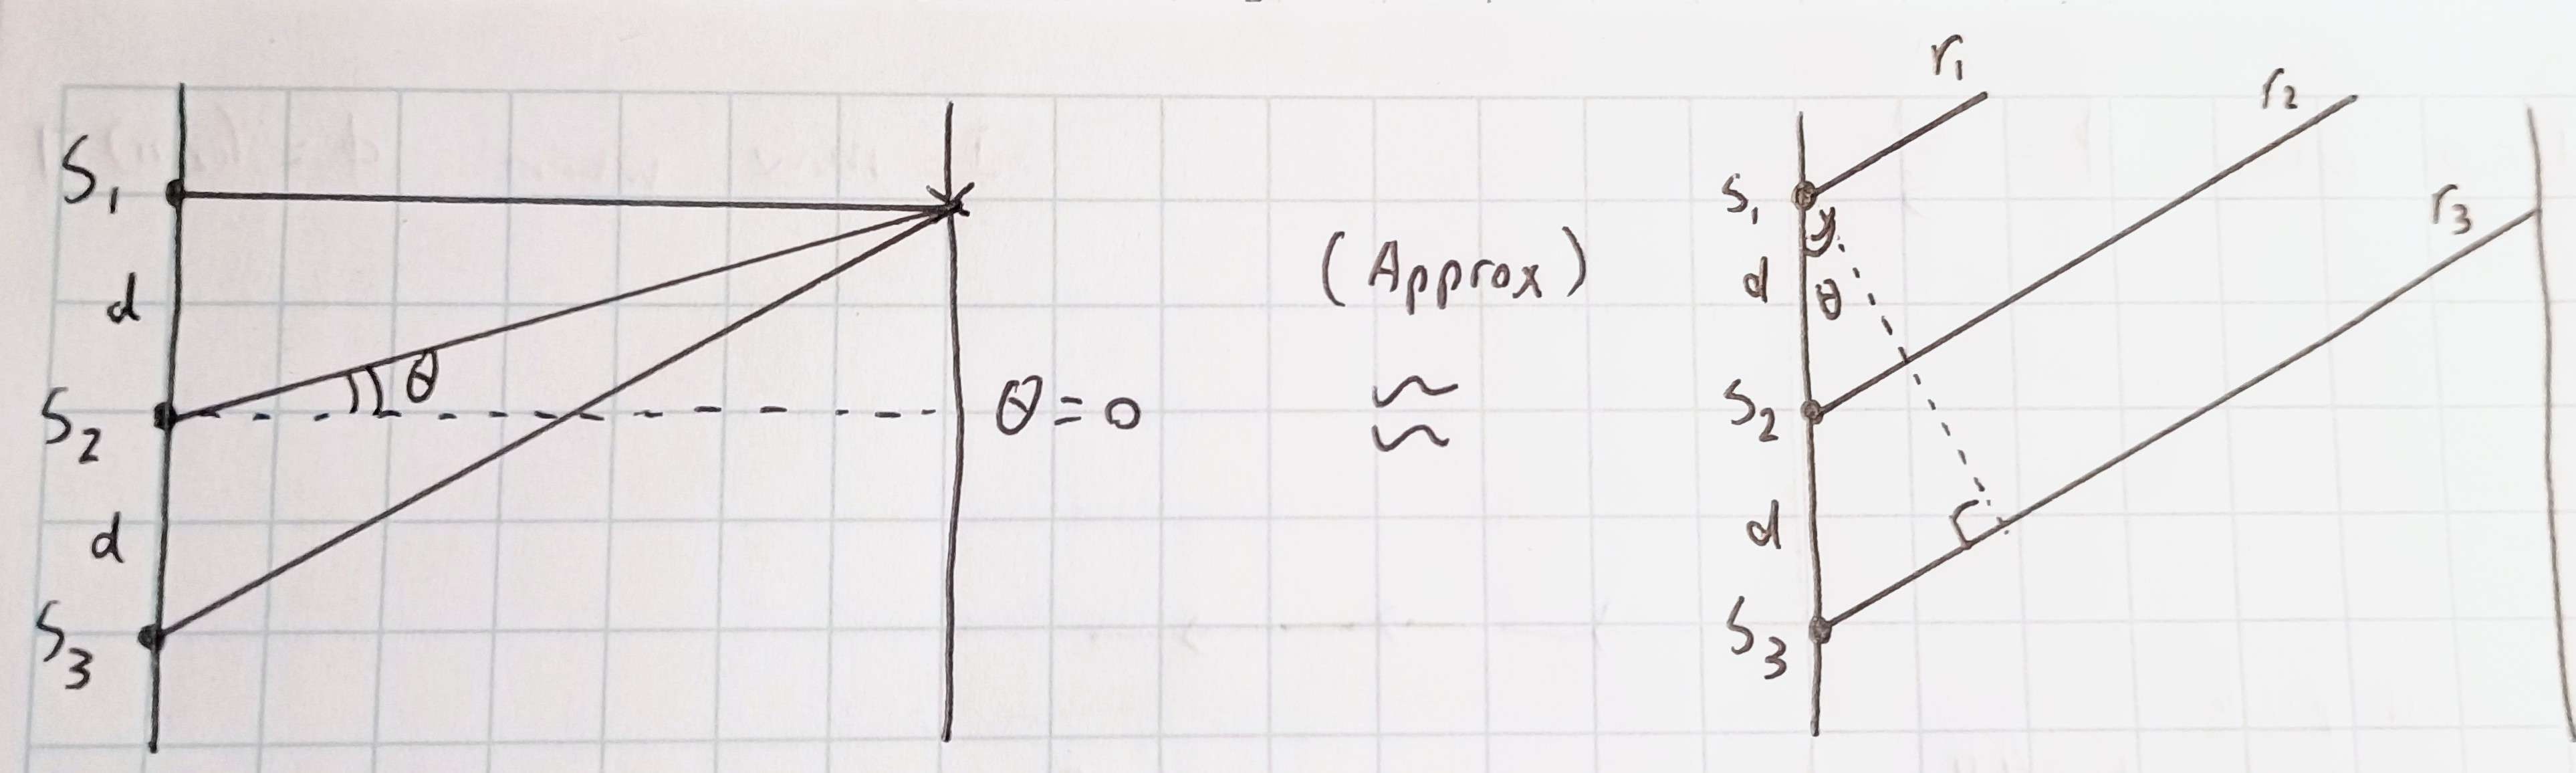
\includegraphics[width=0.8\textwidth]{Triple slit.jpg}
\end{figure}
\[r_2-r_1=dsin\theta\]
\[r_3-r_1=2dsin\theta\]
Thus $y_2$ and $y_3$ are phase shifted from $y_1$
\[y_1=Acos(kx-\omega t)\]
\[y_2=Acos(kx-\omega t+kdsin\theta)\]
\[y_3=Acos(kx-\omega t+2kdsin\theta)\]
\[y_1+y_2+y_3=Ae^{i(kx-\omega t)}\left( 1+e^{ikdsin\theta}+e^{i2kdsin\theta}\right)\]
\begin{figure}[H]
    \centering
    \includegraphics[width=0.8\textwidth]{{Phasor.jpg}}
\end{figure}
\[\lVert y_1+y_2+y_3 \rVert = \sqrt{(1+cos(kdsin\theta)+cos(2kdsin\theta))^2+(sin(kdsin\theta)+sin(2kdsin\theta))^2}\]
Let $\alpha$ be the phase shift of the superposition
\[\alpha = arctan\left( \frac{(kdsin\theta)+sin(2kdsin\theta)}{1+cos(kdsin\theta)+cos(2kdsin\theta)}\right)\]
\[y_1+y_2+y_3 = A\lVert y_1+y_2+y_3 \rVert \operatorname{Re}(e^{i(kx-\omega t+\alpha)})\]
\[y_1+y_2+y_3 = A\lVert y_1+y_2+y_3 \rVert cos(kx-\omega t+\alpha)\]
The intensity as a function of $\theta$ is
\[I = (A\lVert y_1+y_2+y_3 \rVert)^2\]
\[I = A^2\left[(1+cos(kdsin\theta)+cos(2kdsin\theta))^2+(sin(kdsin\theta)+sin(2kdsin\theta))^2\right]\]
\begin{figure}[H]
    \centering
    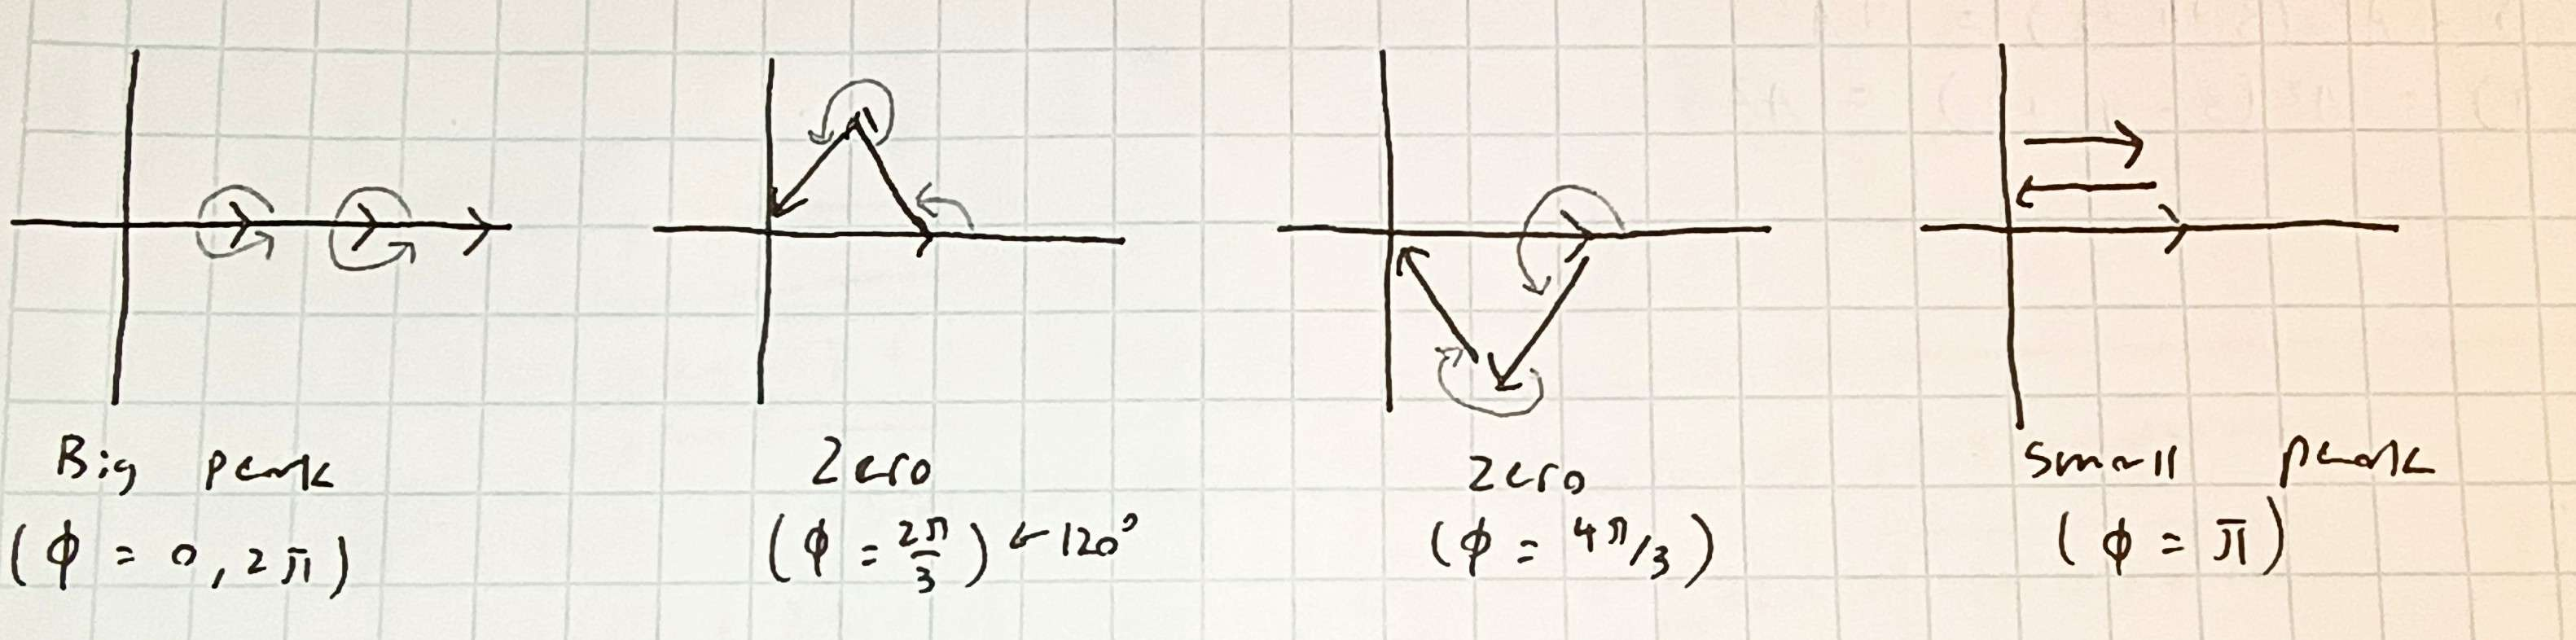
\includegraphics[width=1\textwidth]{MaxMin.jpg}
\end{figure}

    \end{itemize}
\newpage
    \item Find the Fourier series representation for any given periodic function. Describe applications of Fourier analysis. Know the properties of Fourier series. For example, you can reduce the work you need to do for odd versus even functions.\\\\
    (Almost) any periodic f(x) with period $\lambda$ can be written as a fourier series:
    \[f(x)=\frac{A_o}{2}+\sum_{m=1}^{\infty} A_m cos\left(\frac{2\pi}{\lambda}mx\right)+\sum_{m=1}^{\infty} B_n sin\left(\frac{2\pi}{\lambda}mx\right)\]
    Where
    \[A_o = \frac{2}{\lambda}\int_0^\lambda f(x)\,dx=2\cdot\text{(Average value of f(x))}\]
    \[A_n = \frac{2}{\lambda}\int_0^\lambda f(x)cos\left(\frac{2\pi}{\lambda}mx\right)\,dx\]
    \[B_n=\frac{2}{\lambda}\int_0^\lambda f(x)sin\left(\frac{2\pi}{\lambda}mx\right)\,dx\]
    \underline{Note:} Bounds of intergration don't have to start at 0 but has to cover 1 full period.\\
    \underbar{Recall:} Odd fxn: f(-x)=-f(x), even fxn: f(-x)=f(x). \\($\text{Even}\times\text{Even}=\text{Even},\;\text{Odd}\times\text{Odd}=\text{Even},\;\text{Even}\times\text{Odd}=\text{Odd}$)\\\\
\textbf{Even functions only have cosine terms, odd functions only have sine terms}\\\\
\underline{Ex:} Fourier series of $f(x)=|x|$ with $-\pi<x<\pi$ and repeating

\[
f(x) = |x|, \quad x \in (-\pi,\pi) \implies \lambda = 2\pi
\]

\[
f(x) =
\begin{cases}
 -x, & -\pi < x < 0 \\
 x, & 0 < x < \pi
\end{cases}
\]

\[
A_0 = \frac{2}{2\pi} \left[ \int_{-\pi}^{0} -x \, dx + \int_{0}^{\pi} x \, dx \right]
= \frac{1}{\pi} \left[ -\tfrac{1}{2}x^2 \Big|_{-\pi}^{0} + \tfrac{1}{2}x^2 \Big|_{0}^{\pi} \right]
= \frac{1}{\pi} \left[ (0 - -\tfrac{1}{2}\pi^2) + (\tfrac{1}{2}\pi^2 - 0) \right] = \pi
\]

\[
A_n = \frac{2}{2\pi} \left[ \int_{-\pi}^0 -x \cos(mx)\, dx + \int_{0}^\pi x \cos(mx)\, dx \right]
\]

---

Using Integration by parts
\[
\int x \cos(mx)\, dx = \tfrac{x}{m}\sin(mx) - \tfrac{1}{m}\int \sin(mx)\, dx 
= \tfrac{x}{m}\sin(mx) + \tfrac{1}{m^2}\cos(mx)
\]
So
\[
\int_{-\pi}^0 -x\cos(mx)\, dx = -\left[\tfrac{x}{m}\sin(mx) + \tfrac{1}{m^2}\cos(mx)\right]_{-\pi}^0 = \left(- \tfrac{1}{m^2}\right)
- \left(\tfrac{-\pi}{m}\sin(-m\pi) - \tfrac{1}{m^2}\cos(-m\pi)\right)
\]
\[
\int_{0}^\pi x\cos(mx)\, dx = \left[\tfrac{x}{m}\sin(mx) + \tfrac{1}{m^2}\cos(mx)\right]_{0}^\pi = \left(\tfrac{\pi}{m}\sin(m\pi) + \tfrac{1}{m^2}\cos(m\pi)\right)-\left(\tfrac{1}{m^2}\right)
\]
---

\[
A_n = \frac{1}{\pi}\Bigg[ \Big(-\tfrac{1}{m^2}\Big) - \Big(\tfrac{-\pi}{m}\sin(-m\pi) - \tfrac{1}{m^2}\cos(-m\pi)\Big) 
+ \Big(\tfrac{\pi}{m}\sin(m\pi) + \tfrac{1}{m^2}\cos(m\pi)\Big) - \Big(\tfrac{1}{m^2}\Big)\Bigg]
\]

\[
= \frac{1}{\pi}\Big[\tfrac{2}{m^2}\cos(m\pi) - \tfrac{2}{m^2} \Big]
\]

\[
= \frac{2}{\pi}\Big( \tfrac{1}{m^2}(-1)^m - \tfrac{1}{m^2} \Big)
= \frac{2}{\pi m^2}\left((-1)^m - 1\right)
\]

\[
B_n = 0 \quad (\text{$f(x)$ is even})
\]

So the Fourier series is:

\[
f(x) = |x| \approx \frac{\pi}{2} + \sum_{m=1}^\infty \frac{2}{\pi m^2}\left((-1)^m - 1\right)\cos(mx)
\]

For \(m\) even: \((-1)^m - 1 = 0\). \\ 
For \(m\) odd: \((-1)^m - 1 = -2\).

So let $m=2k-1$:

\[f(x) \approx \frac{\pi}{2} - \frac{4}{\pi} \sum_{k=1}^\infty \frac{\cos((2k-1)x)}{(2k-1)^2} \]

\newpage

    \item Know, qualitatively, what makes dispersive waves, like water waves, different from linear waves, like waves on a string. This includes the definition of dispersion as applied to waves and the distinction between phase and group velocity.\\\\
    Unlike linear waves, dispersive waves are a superposition of waves that breaks apart as it propagates. (Ex: Water waves with $v_w=\sqrt{g\lambda}$ so longer wavelength waves will spread out more)
    \begin{itemize}
        \item Phase velocity: speed of individual wave fronts
        \[v_{phase}=\frac{\omega}{k}\]
        \item Group velocity: the speed of a traveling interference pattern (the overall shape), sometimes called a wave packet. (Ex: the "beat" velocity)
        \[v_{group}=\frac{d\omega}{dk}\]
        \underline{Ex:} Water waves
        \[v_w=\frac{\omega}{k}=\sqrt{\frac{g\lambda}{2\pi}}\]
        \[\omega=\sqrt{gk}\]
        \[v_{group}=\frac{d\omega}{dk}=\frac{1}{2}\sqrt{\frac{g}{k}}\]
    \end{itemize}
    \newpage
    \item Misc.
    \begin{itemize}
        \item Supersonic shock waves\\
        When an object moves faster than the speed of sound, it forms a mach cone with a mach cone angle:
        \[sin\theta =\frac{v_{sound}t}{v_{source}t}=\frac{v_{sound}}{v_{source}}\]
        Where t is the time elapsed between the emission of wave fronts
        \[\text{Mach Number}=\frac{v_{source}}{v_{sound}}\]
        \begin{figure}[H]
    \centering
    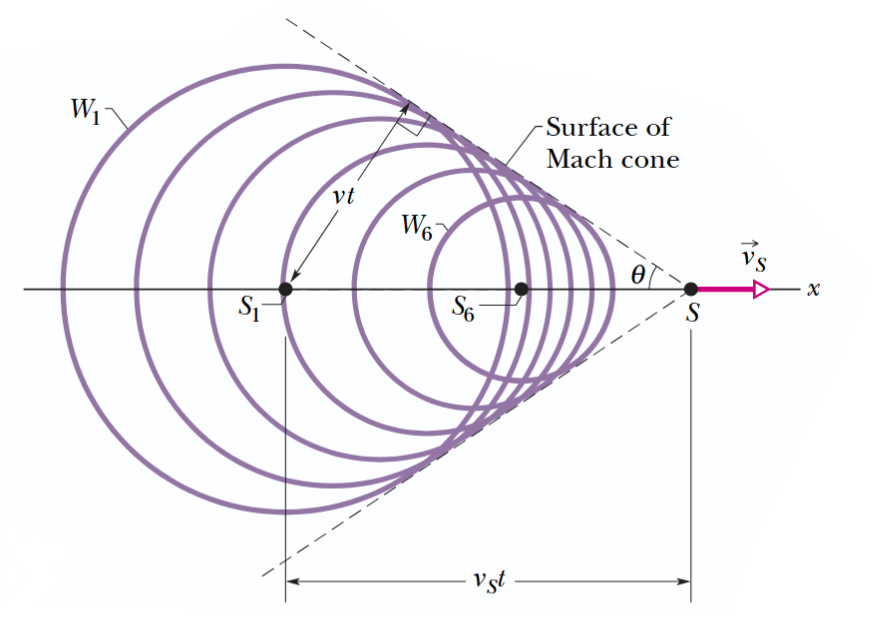
\includegraphics[width=0.7\textwidth]{mach cone.png}
        \end{figure}
    \end{itemize}
    
\end{enumerate}

\textbf{End Exam 1}



\end{document}